\documentclass[final,hyperref={pdfpagelabels=false}]{beamer}
\usepackage[orientation=landscape,size=a0,scale=1.6]{beamerposter}
\usecolortheme{seahorse}
\useinnertheme{rounded}
\setbeamertemplate{navigation symbols}{}
\setbeamertemplate{footline}{}

\definecolor{CranfieldBlue}{RGB}{0,51,102}
\setbeamercolor{title}{fg=CranfieldBlue}
\setbeamercolor{author}{fg=black}
\setbeamercolor{institute}{fg=black}
\setbeamercolor{block title}{bg=CranfieldBlue,fg=white}
\setbeamercolor{block body}{bg=white,fg=black}

\usepackage{graphicx}
\usepackage{booktabs}
\usepackage{amsmath,amssymb}
\usepackage[utf8]{inputenc}
\usepackage{tikz}
\usetikzlibrary{arrows.meta,positioning,shapes.geometric}

\title{From Measured Pore-Scale Operators to Network-Level Prediction in a Structured Belousov--Zhabotinsky Reactor}
\author{Srivijayesh Venugopal}
\institute{Supervisor: Prof. Weisi Guo\\Cranfield University, MSc Computational Fluid Dynamics}

\newcommand{\email}[1]{}

\begin{document}
\begin{frame}[t]{}

\begin{columns}[T]

% ---------------------------------------------------------------------------
% Column 1: big picture
% ---------------------------------------------------------------------------
\begin{column}{0.31\paperwidth}

\begin{block}{Idea}
Digital inference is limited by the von Neumann bottleneck. Physical neural networks use the material itself as the computer: excitations are inputs, structure is the program, and probes read outputs.
\end{block}

\begin{block}{Porous reactor as a physical computer}
\centering
\begin{tikzpicture}[node distance=0.9cm, every node/.style={align=center, font=\footnotesize}]
\node[draw, rounded corners, fill=CranfieldBlue!10, text width=4.0cm] (macro) {Porous BZ reactor};
\node[draw, rounded corners, fill=CranfieldBlue!10, text width=4.0cm, below=of macro] (micro) {2D BZ calibration};
\node[draw, rounded corners, fill=CranfieldBlue!10, text width=4.0cm, below=of micro] (graph) {Graph simulator};
\draw[-{Stealth}, thick] (macro) -- node[right]{calibrate} (micro);
\draw[-{Stealth}, thick] (micro) -- node[right]{compose} (graph);
\draw[-{Stealth}, thick, dashed] (graph.west) -- ++(-1.2,0) |- (macro.west);
\end{tikzpicture}

\vspace{0.3cm}
A real 3D pore network is too fine to resolve. We abstract pores as nodes and throats as edges, then calibrate each element with 2D simulations.
\end{block}

\begin{block}{Why BZ reaction--diffusion?}
\begin{itemize}
\item Acoustic waves: no native nonlinearity.
\item Well-mixed CRNs / DNA: no spatial structure.
\item BZ offers self-sustaining pulses, collision/annihilation, refractory inhibition, and optical control via a photosensitive catalyst.
\end{itemize}
\end{block}

\begin{block}{Model}
Two-variable Tyson--Fife Oregonator with light suppression:
\begin{equation*}
\frac{\partial u}{\partial t} = \frac{1}{\varepsilon}\left[u-u^2-(fv+\phi)\frac{u-q}{u+q}\right]+\nabla\!\cdot\!(\mathbf{D}\nabla u),\qquad
\frac{\partial v}{\partial t} = u-v.
\end{equation*}
\end{block}

\begin{figure}
\centering
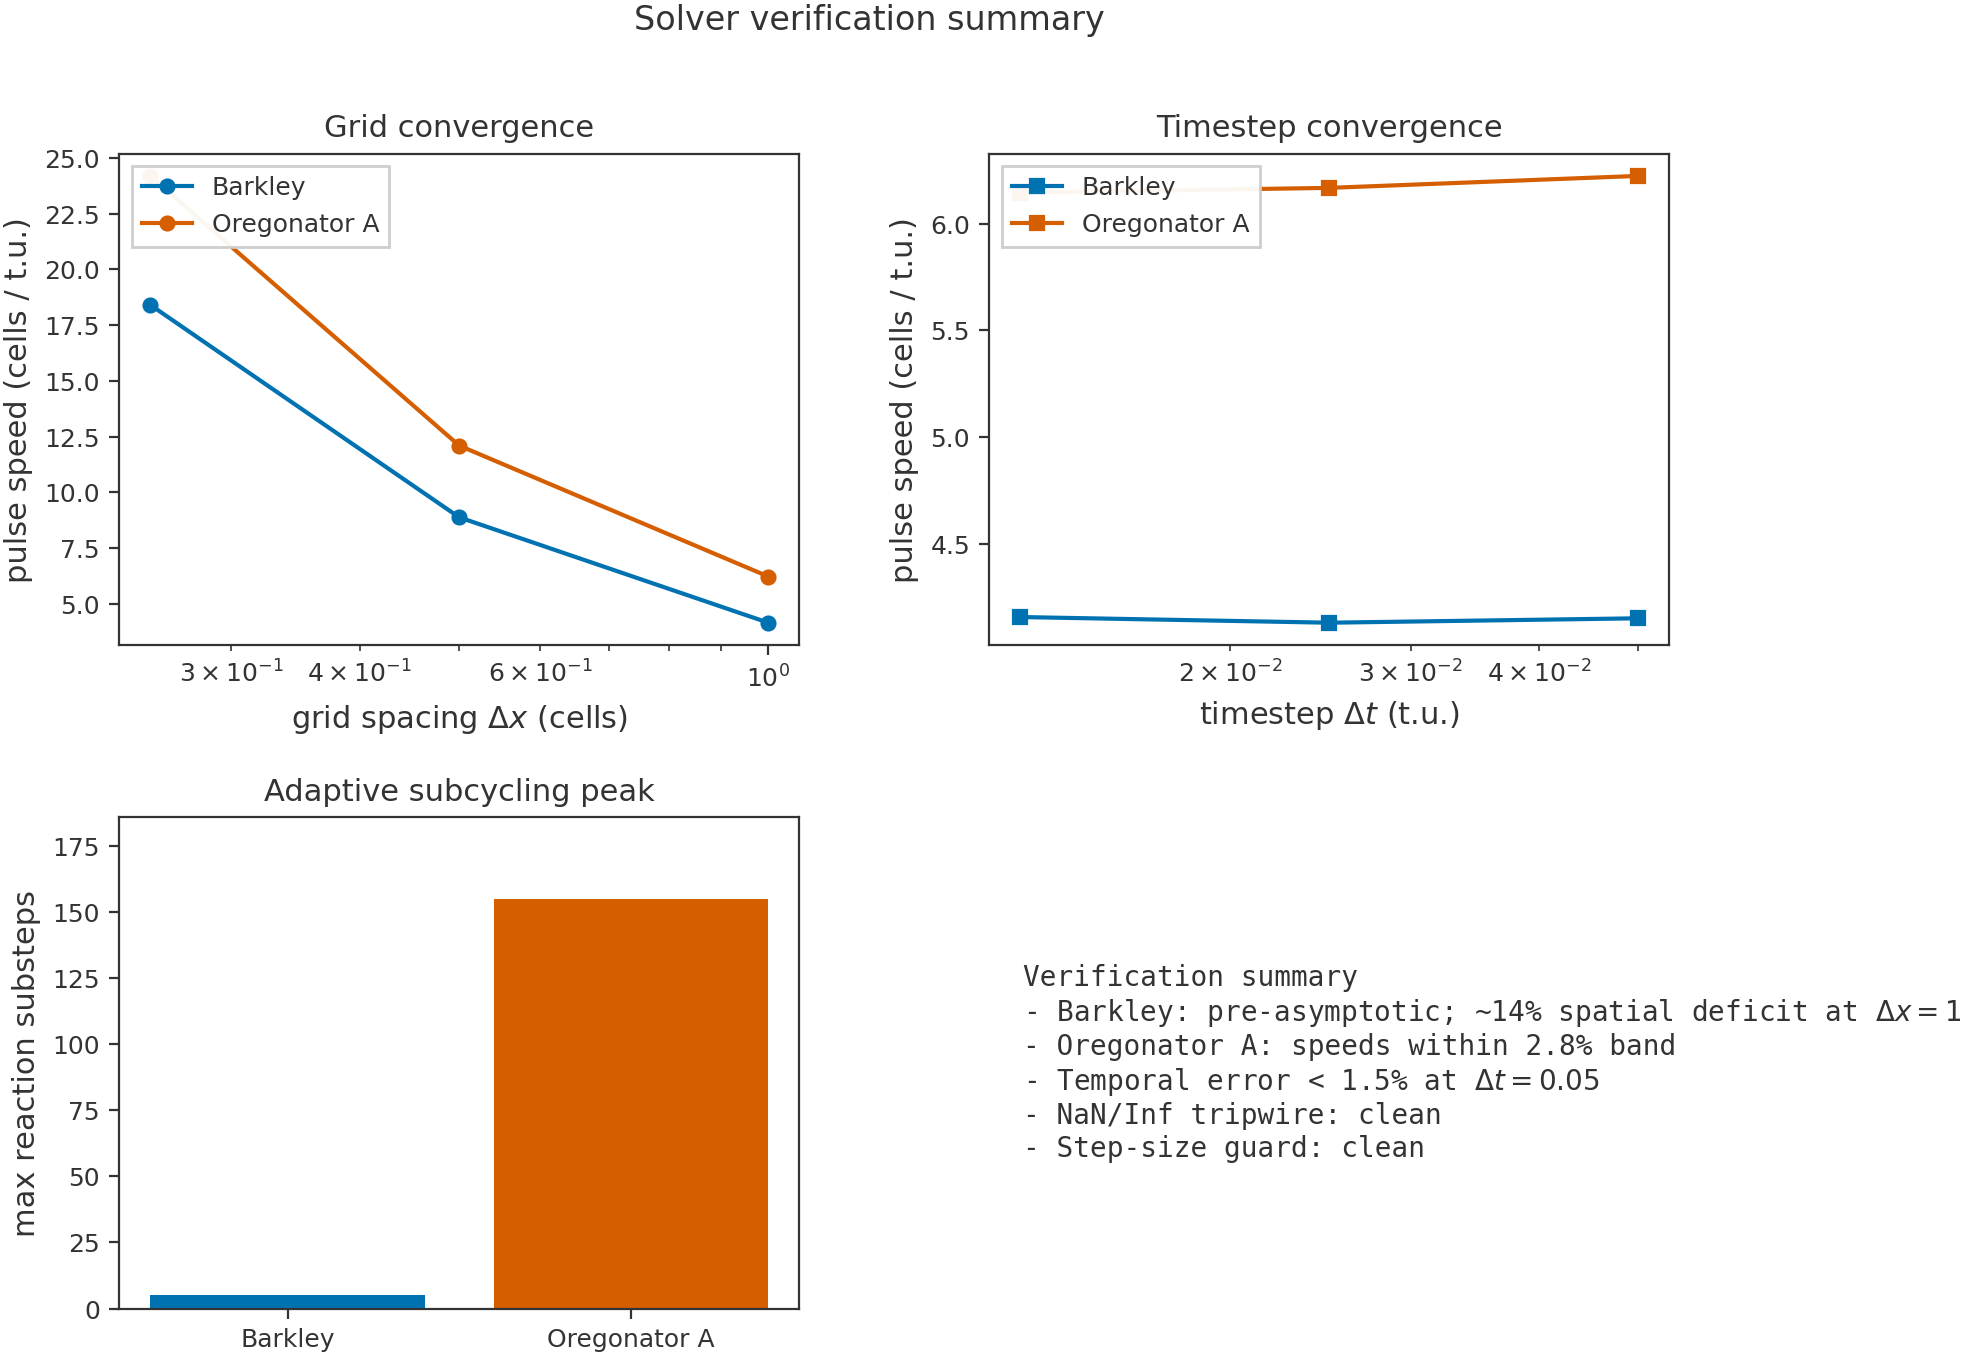
\includegraphics[width=0.95\columnwidth]{../Analysis/figures/pub/pub_verification.png}
\caption{Solver verification against canonical BZ phenomenology.}
\end{figure}

\end{column}

% ---------------------------------------------------------------------------
% Column 2: measured operators (visual)
% ---------------------------------------------------------------------------
\begin{column}{0.31\paperwidth}

\begin{block}{Four measured pore-scale operators}
A black-box dark-spot protocol isolates the native instruction set of the substrate.
\end{block}

\begin{figure}
\centering
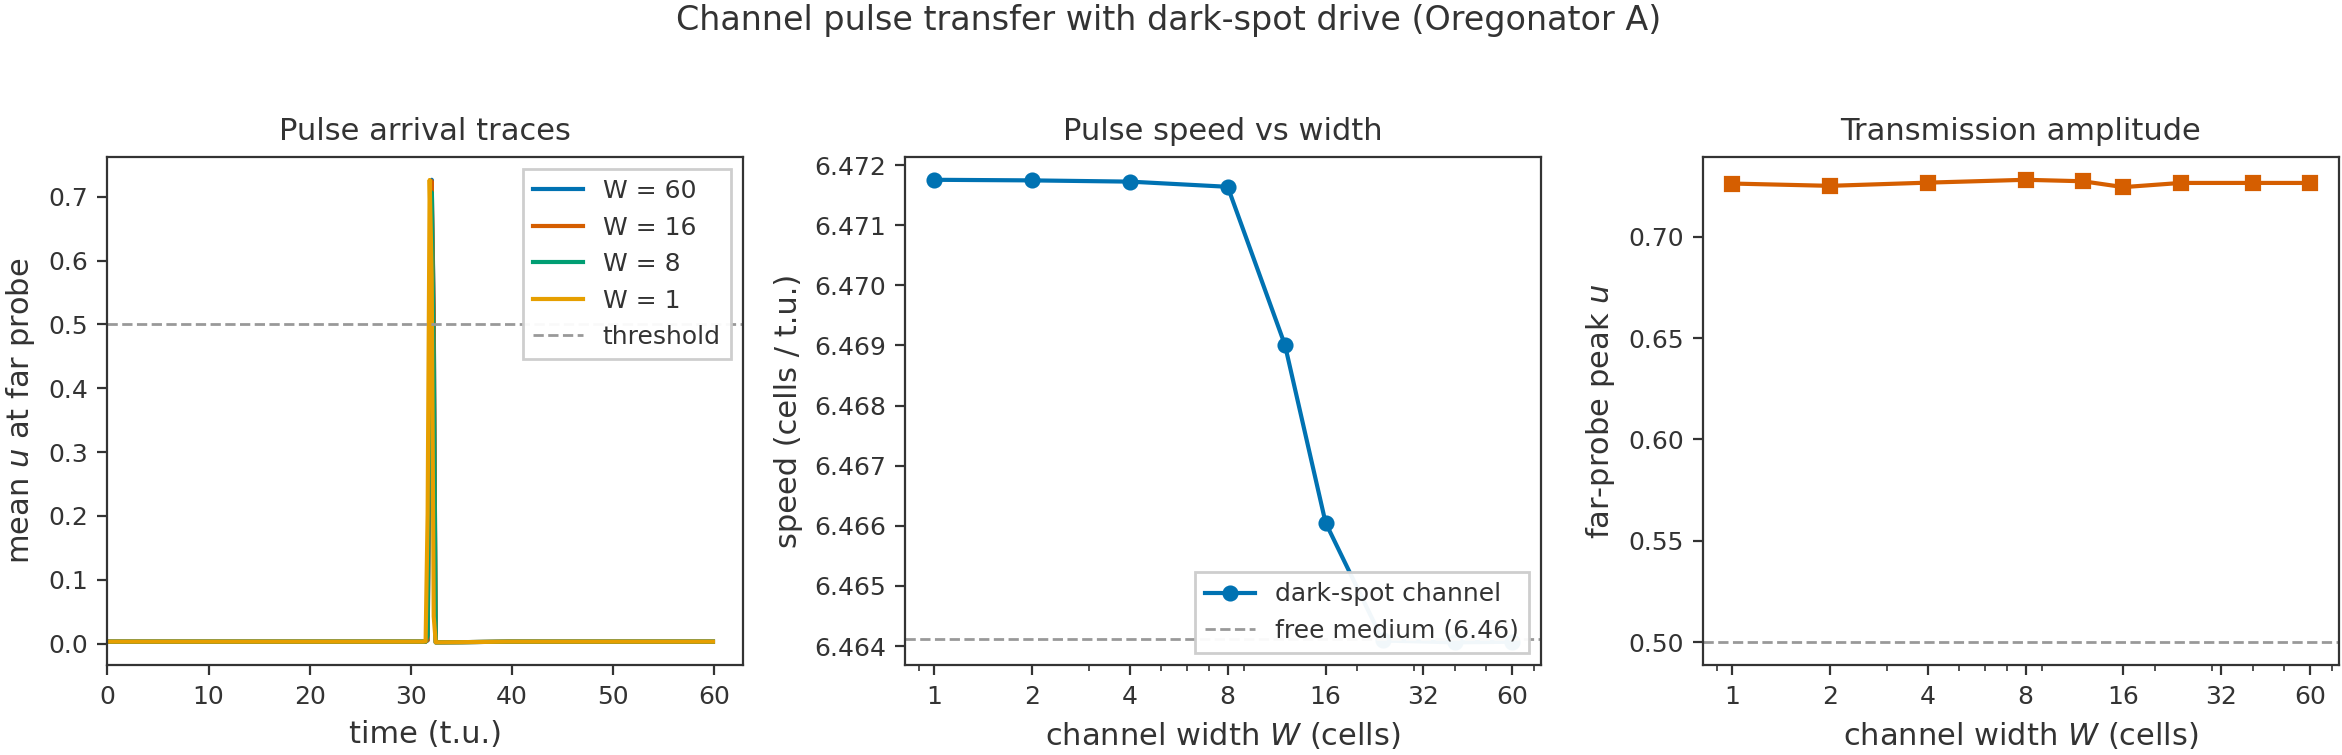
\includegraphics[width=0.95\columnwidth]{../Analysis/figures/pub/pub_channel_transfer_darkspot.png}
\caption{\textbf{Wire:} speed is independent of width. 2D $6.46 \pm 0.19$, 3D $6.62 \pm 0.20$ cells/t.u.}
\end{figure}

\begin{figure}
\centering
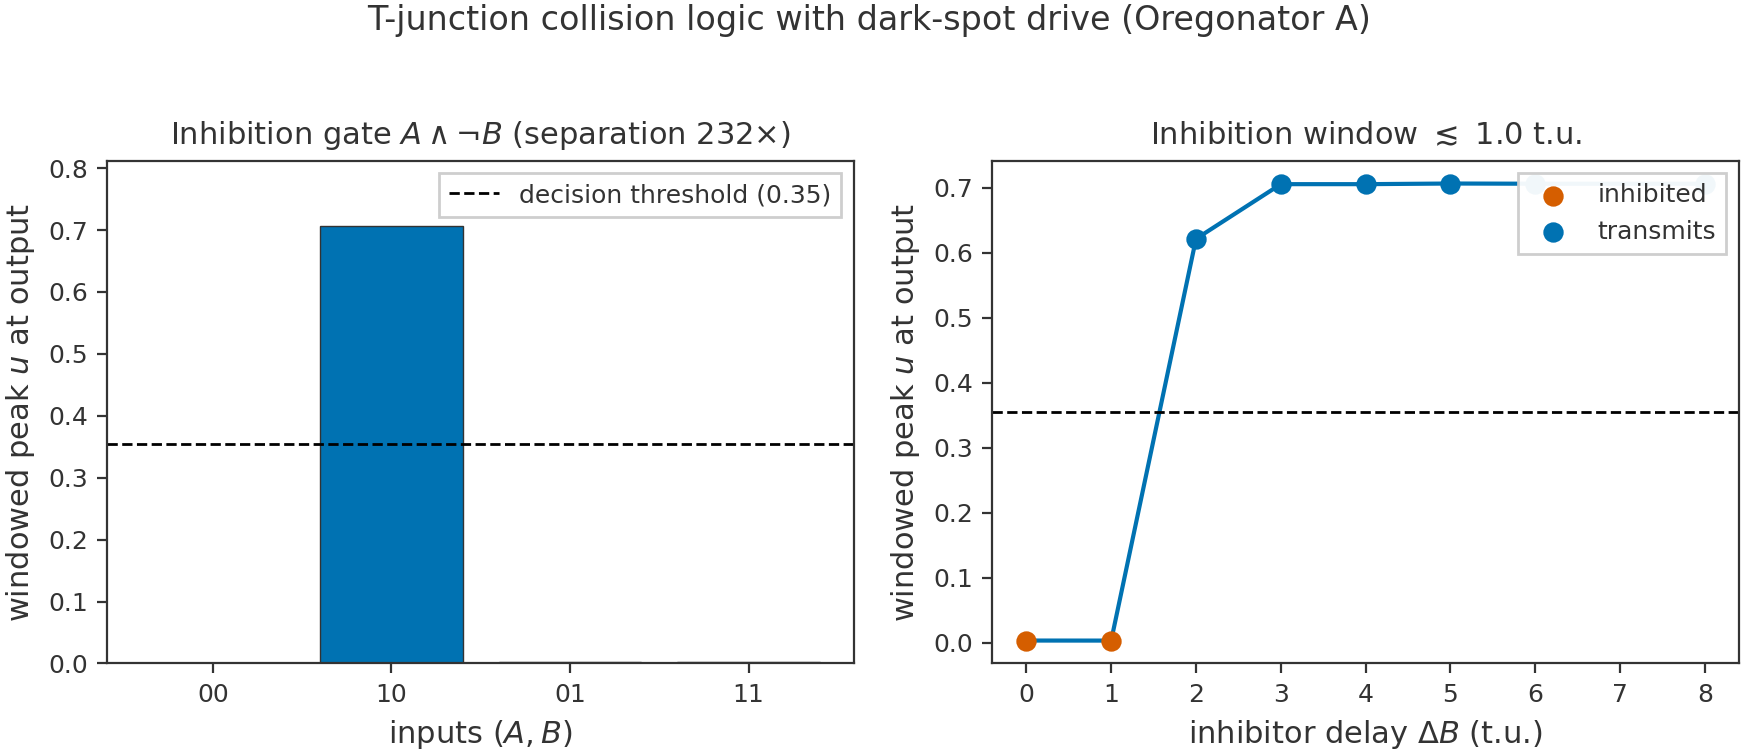
\includegraphics[width=0.95\columnwidth]{../Analysis/figures/pub/pub_tjunction_logic_darkspot.png}
\caption{\textbf{Inhibition gate:} A AND (NOT B) with separation $>100\times$.}
\end{figure}

\begin{figure}
\centering
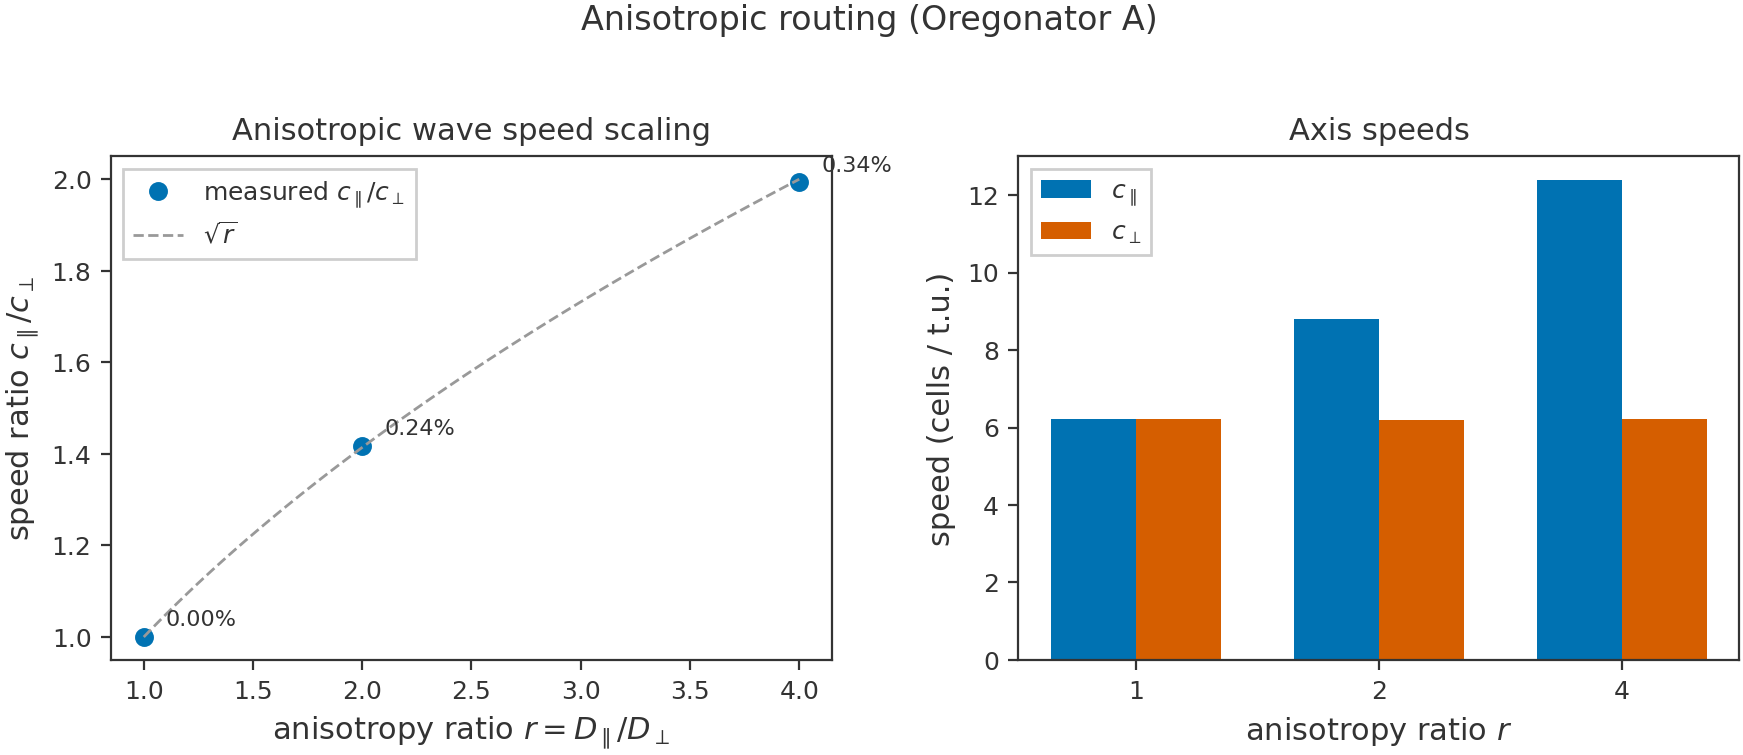
\includegraphics[width=0.95\columnwidth]{../Analysis/figures/pub/pub_anisotropic_routing.png}
\caption{\textbf{Anisotropic routing:} elliptical fronts follow the eikonal $\sqrt{r}$ speed law.}
\end{figure}

\begin{block}{Frequency limit}
Absolute refractory period: $3.0 \pm 0.1$ t.u.; max 1:1 following rate: $0.167$ t.u.$^{-1}$.
\end{block}

\end{column}

% ---------------------------------------------------------------------------
% Column 3: composition and conclusions
% ---------------------------------------------------------------------------
\begin{column}{0.31\paperwidth}

\begin{block}{From operators to networks}
Measured transit times, refractory windows, and inhibition rules become an event-driven graph simulator. It predicts pulse traffic in milliseconds before an expensive PDE run.
\end{block}

\begin{figure}
\centering
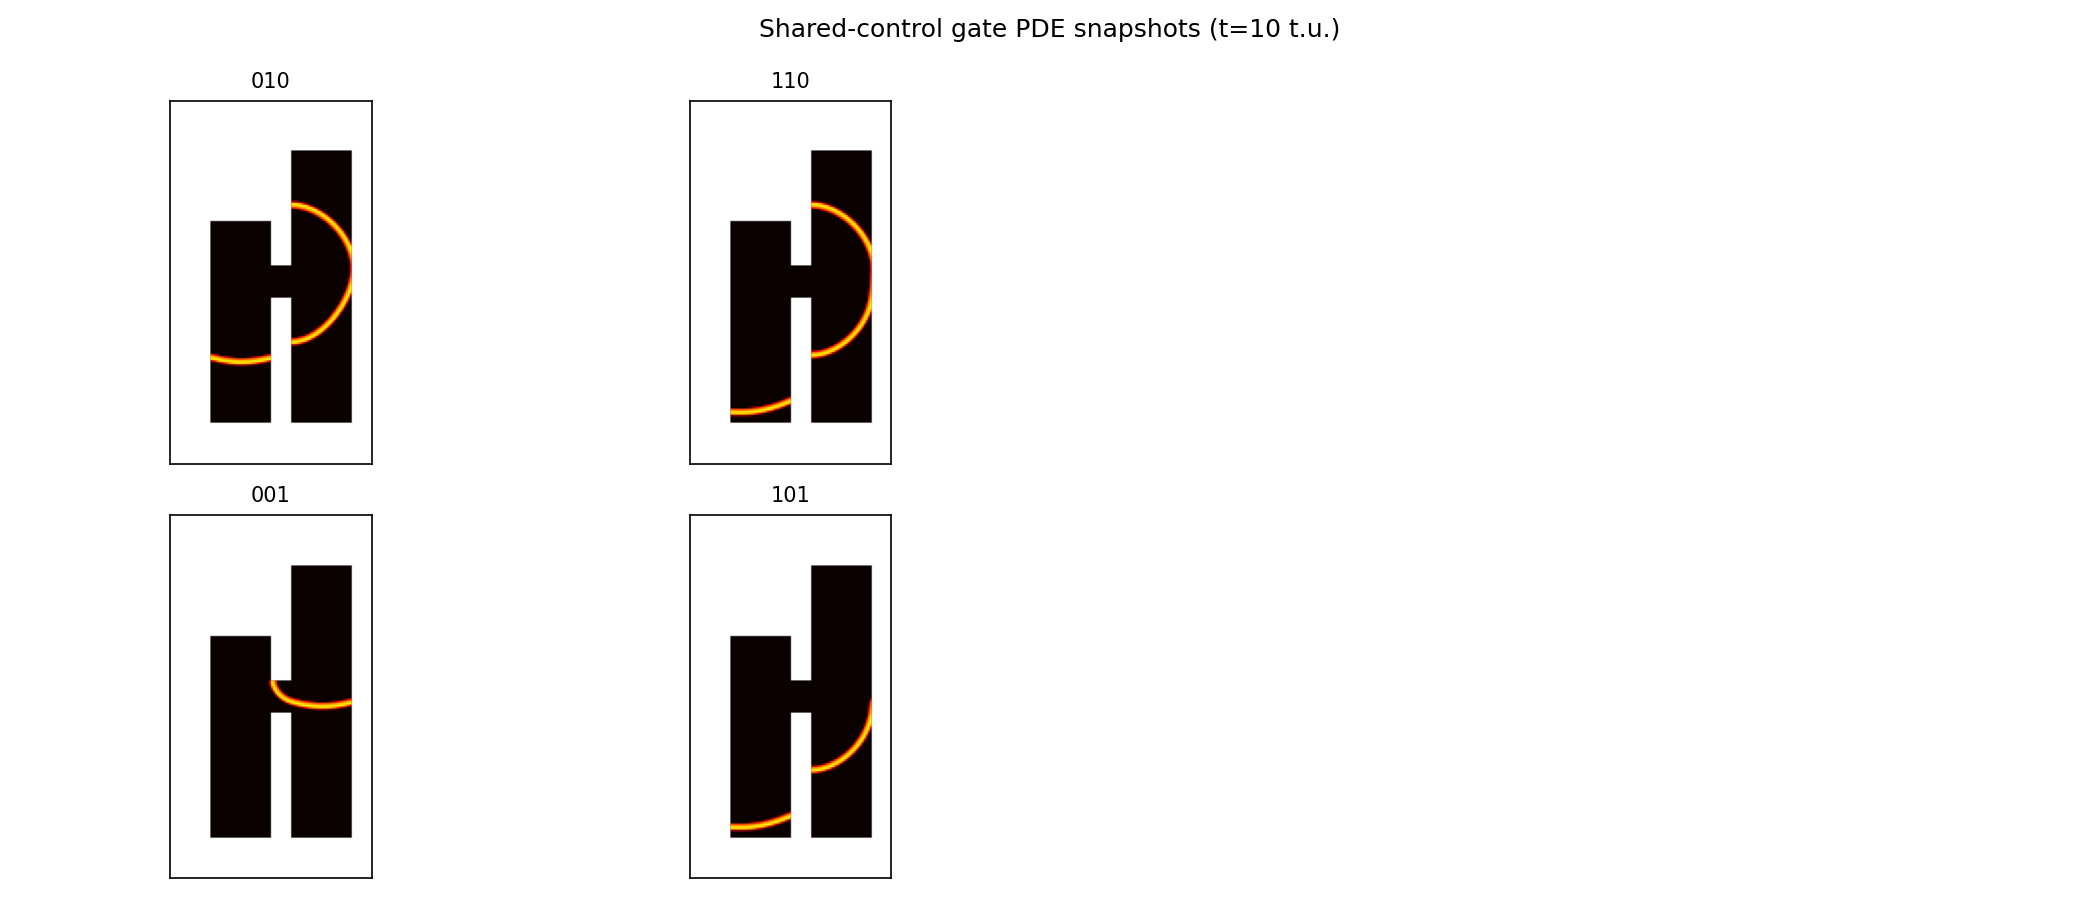
\includegraphics[width=0.46\columnwidth]{../Analysis/figures/rd_multi_gate_pde_snapshots.png}
\hfill
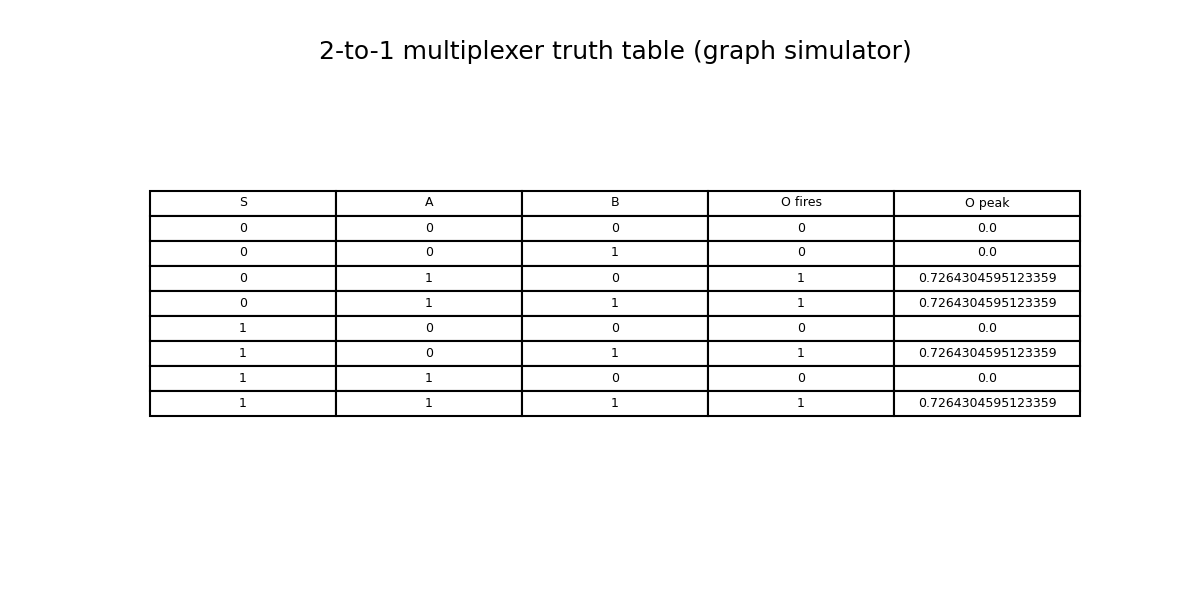
\includegraphics[width=0.46\columnwidth]{../Analysis/figures/rd_mux_graph.png}
\caption{Left: shared-control multi-junction gate. Right: graph-simulator 2-to-1 MUX.}
\end{figure}

\begin{block}{What transfers to 3D?}
\begin{itemize}
\item \textbf{Works:} thin-slab 3D inhibition gate ($16.8\times$ separation).
\item \textbf{Boundary result:} 3D MUX needs better geometry; S does not yet block A cleanly.
\item \textbf{Does not work:} simple asymmetric diode or static light barrier.
\end{itemize}
\end{block}

\begin{figure}
\centering
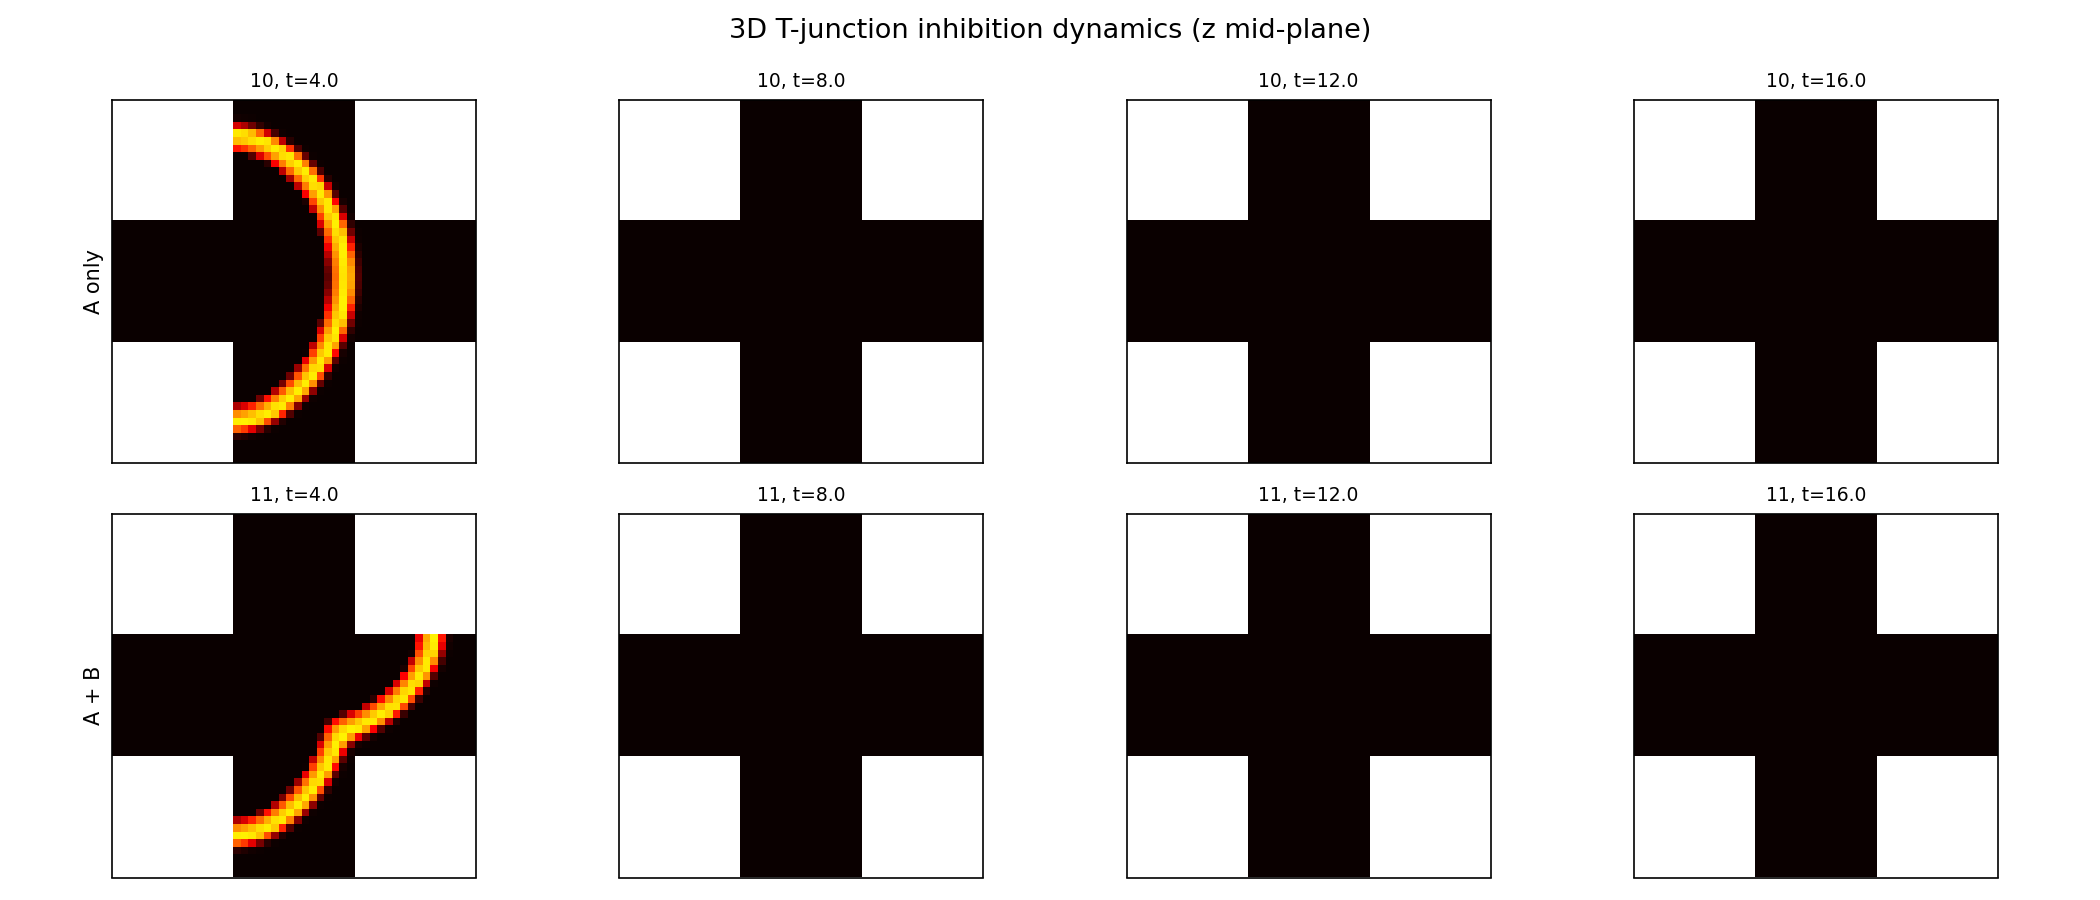
\includegraphics[width=0.46\columnwidth]{../Analysis/figures/rd_3d_transfer_logic_snapshots.png}
\hfill
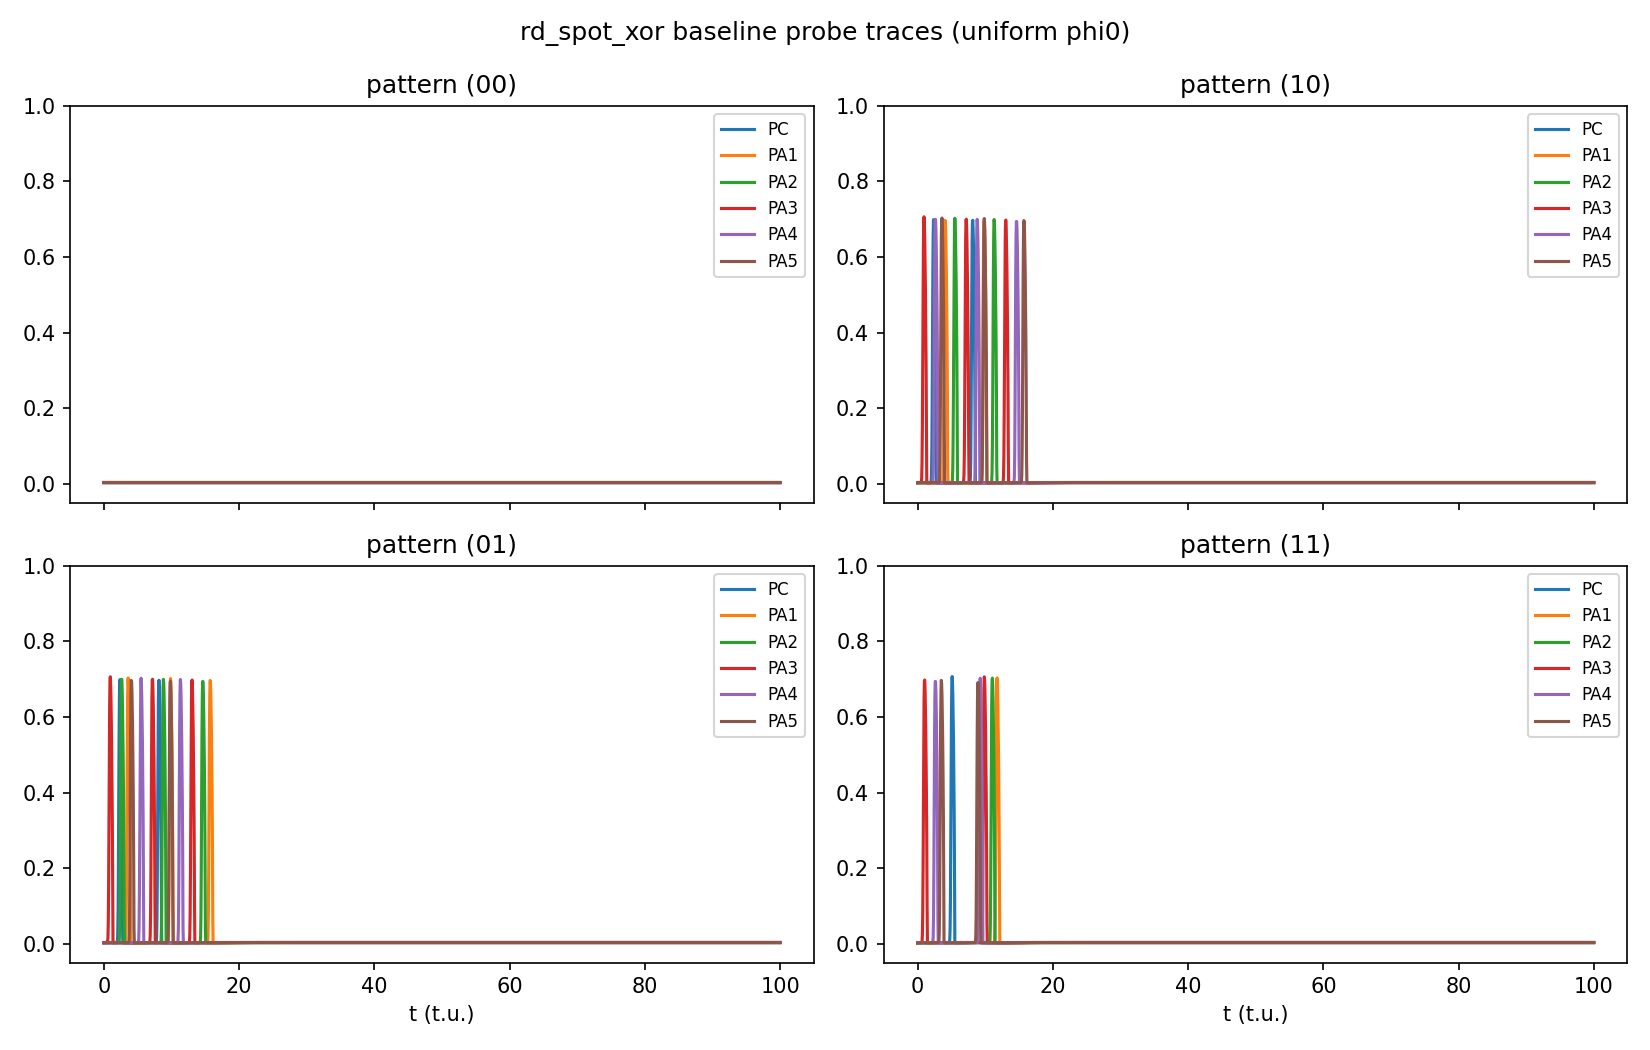
\includegraphics[width=0.46\columnwidth]{../Analysis/figures/rd_spot_xor_protocol.png}
\caption{Left: 3D inhibition gate. Right: collision XOR leaks.}
\end{figure}

\begin{block}{Take-away}
Network-level pulse routing in a structured excitable medium can be predicted from micro-scale transfer functions, but only when each junction geometry is carried explicitly in the model.
\end{block}

\begin{block}{Next steps}
Shape-resolved junction library, volumetric 3D illumination strategy, and experimental calibration.
\end{block}

\end{column}

\end{columns}

\end{frame}
\end{document}
